\section{Upgrading the consensus layer}

Our construction requires an upgrade to the bitcoin consensus layer. In this
section we outline a possible upgrade path for the bitcoin network. The obvious
path forward for implementing our construction requires building an altcoin or
a hard fork for the new construction. This is the path implied in
\cite{KLS}.

Nevertheless, it is not hard to see that an existing coin such as bitcoin can
be upgraded to work with the new consensus rules using a soft fork.  Such a
construction in practice would require including the interlink data structure
not in the block header, but in the data of the coinbase transaction.  Clearly
it is enough to store a single hash of the whole interlink structure in the
coinbase data. The only requirement for the PoPoWs to work is that the
PoW commits to all the pointers within interlink so that the adversary cannot
cause a chain reorganization except with negligible probability. That way, each
superchain is really a chain which goes all the way back to genesis. If we take
that route, then each PoPoW will be required to present not only the block
header, but also a proof-of-inclusion path within the Merkle tree of
transactions proving that the coinbase transaction is indeed part of the block.
Once that is established, the coinbase data can be presented, and the verifier
will thereby know that the hash of the interlink data structure is correct.
Given the fact that in the current bitcoin implementation there is a fixed
limit for block sizes, we observe that including such proofs-of-inclusion will
only increase the PoPoW sizes by a constant factor per block, allowing for the
communication complexity to remain at $\Theta(polylog(|\chain|))$.

We now discuss the exact manner in which the interlink data structure should be
hashed to provide a single hash within the coinbase transaction. In \cite{KLS},
they propose the use of a Merkle tree to hash the interlink data structure.
However, no further discussion is made in this regard. However, observe that
whenever a block $B$ is included in a NIPoPoW and provided a superblock pointer
of level $i$ is needed to point from block $B$ to a previous block, then
we necessarily have that all the superblock pointers of level $i + j$ for
positive $j$ will also have to be included. The one exception to this is only
for blocks that are the oldest ones to be included from each superchain. Given
that the maximum superblock level of a superchain containing at least $m$
blocks is $\mu$, we know that these exceptional blocks will only be $\mu$. The
second exception is in regards to pointers of very high superblock levels that
have not yet been able to form a superchain of length at least $m$. The count
of these blocks will be $log(m)$ in expectation. Given that the total number of
blocks presented in a NIPoPoW are $2m\mu - m$ in expectation, we observe that
for the majority of blocks in a NIPoPoW proof we need to present a prefix of
the interlink structure containing pointers of a certain superblock level and
above, of which only very few very high-level pointers are unnecessary.
Therefore, it makes sense to optimize the storage of interlink in such a way
that the NIPoPoW can shortly present only the necessary prefix of interlink.

The way to do that is by collecting the interlink data structure in a
completely imbalanced binary Merkle tree which simply constitutes a Merkle
chain. Note that the level 0 pointer is included in the block header as usual,
so it does not need to be included here. The tree is constructed by initially
taking the two lowest levels of superblock pointers, level 1 and 2 and
combining them as leaves of a single parent. For each next level, the previous
level parent is taken as a child of a new parent also containing the next level
as a leaf, as seen in Figure~\ref{fig.merkle_chain}, forming a chain. The hash
of the Merkle chain root (marked gray in the figure) is then included in the
coinbase transaction data.

Whenever a Prover wishes to present superblock pointers of the top $i$ levels,
they only need to present the $i$ pointers themselves as well as the
lowest-level sibling in the Merkle chain (marked black in the figure). In that
manner, these proofs are optimal in size, as they only include an additional
constant term, and are $\Theta(i)$ per block.  Traditional balanced Merkle
trees would require a $\Theta(i + log(\mu))$ per block for the presentation of
the interlink data structure.

\begin{figure}[h]
    \caption{\label{fig.merkle_chain}
    A Merkle chain hashing the interlink data structure for short
    proof sizes. The gray root node hash is included in the coinbase
    transaction. Here, the prover wishes to present superblock pointers of
    levels 4 and above. They must include the data of the black nodes in their
    proof.}
    \centering
    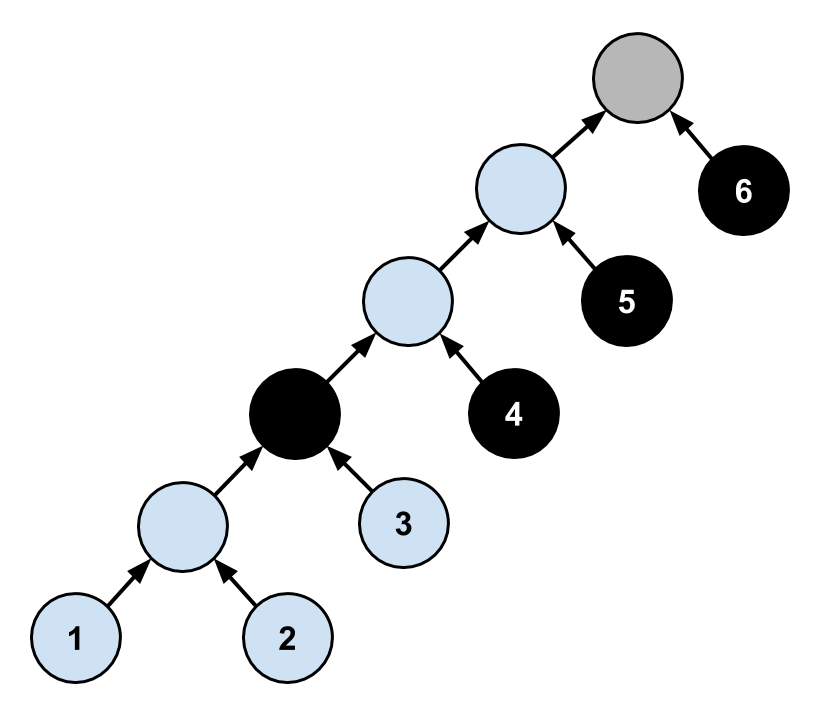
\includegraphics[width=0.3\textwidth,keepaspectratio]{figures/merkle-chain.png}
\end{figure}

Now that the consensus layer details have been presented, we move on to
illustrate that, in fact, no fork is needed. Given that intuitively these
changes constitute rule modifications to the consensus layer, we call this
technique a \textit{velvet fork}.

The way to achieve this is by requiring upgraded miners to include the
interlink data structure in the form of a Merkle chain root hash in their
coinbase data, similar to a soft fork. An unupgraded miner will as usual ignore
this data as comments. However, we further require the upgraded miners to
accept all previously accepted blocks, regardless of whether they have included
the interlink data structure or not. In fact, even if the interlink data
structure is included and contains invalid data, we require the upgraded miners
to accept their containing blocks. Malformed interlink data could be simply of
the wrong format, for example higher-level points appearing lower in the Merkle
chain, or the pointers could be pointing to superblocks of incorrect
levels. Furthermore, the pointers could be pointing to superblocks of the
correct level, but not to the most recent block. By requiring upgraded miners
to accept all such blocks, we do not modify the set of accepted blocks:
Upgraded and unupgraded miners accept the exact same set of blocks. Therefore,
the upgrade is simply a "recommendation" for miners and not an actual change in
the consensus rules.

The reason this can work is because provers and verifiers of our protocol can
check the validity of the claims of miners who make false interlink chain
claims. An upgraded Prover can check whether a block contains correct interlink
data and use it. If a block does not contain correct interlink data, the Prover
can opt not to use those pointers at all in their proofs. As the Verifier
verifies all claims of the Prover, adversarial miners cannot cause harm by
including invalid interlink data. The only thing that the Verifier cannot
verify in terms of interlink claims is whether the claimed superblock of a
given level is in fact the most recent previous superblock of that level.
However, an adversarial Prover cannot make use of that to construct winning
proofs, as they are only able to present shorter chains in that case. The
honest Prover can simply ignore such pointers as if they were not included at
all.

The velvet Prover is shown in Algorithm~\ref{alg.backbone-velvet-prover}. The
Prover works as usual, but additionally mantains a realLink data structure
which stores the correct interlink for each block. Whenever a block is received
from the network, the Prover checks to see if the interlink included in the block is
correct and corresponds to their internal state realLink. If so, these
interlinks are used in the Prover's proofs; otherwise they are ignored.

\import{./}{algorithms/alg.backbone-velvet-prover.tex}
\import{./}{algorithms/alg.nipopow-velvet-innerchain.tex}
